\chapter{Estática estructural}

La Estática es parte de la Mecánica, y ésta es una rama de la Física.
La Física es la ciencia que estudia los diferentes tipos de movimientos de la materia y sus
transformaciones mutuas, así como la estructura y propiedades de las formas concretas de la
materia (sólidos, líquidos, gases y campos). La palabra Física es de origen griego y significa
naturaleza; como ciencia se inicia con Galileo (1564-1642).


La Mecánica es la rama de la Física que estudia las leyes generales del movimiento mecánico (o
simplemente el movimiento) de los cuerpos, y establece los métodos generales para la solución
de los problemas relacionados con este tipo de movimiento. La palabra Mecánica es de origen
griego y significa construcción, máquina o invento; aparece por primera vez en las obras de
Aristóteles (384-322 a.C.).

El movimiento mecánico se refiere a los cambios de posición (desplazamientos) de los cuerpos,
unos con respecto a otros, que suceden en el transcurso del tiempo, así como la variación de la
posición relativa de las partículas de un mismo cuerpo, es decir, la deformación de este último.
El estado de reposo de los cuerpos es un caso especial de movimiento, de cuyo estudio se encarga
la parte de la Mecánica denominada Estática.


Problemas fundamentales de la Mecánica como ciencia.

\begin{enumerate}
	\item El estudio de diferentes movimientos y la generalización de los resultados obtenidos en forma de leyes, con ayuda de las cuales pueda predecirse el carácter del movimiento en cada caso concreto. Así se han establecido, por ejemplo, las leyes y teoremas de la Dinámica y, en particular, de la Estática
	\item La búsqueda de propiedades generales, propias de cualquier sistema, independientemente de la especie concreta de interacción entre los cuerpos de éste. Así se han descubierto las leyes de conservación: de la energía, de la cantidad de movimiento y del momento de la cantidad de movimiento.
\end{enumerate}


¿Cuáles son las divisiones o campos de la Mecánica?

Como ocurre en toda la Física, la clasificación más general de la Mecánica es como sigue:

\begin{figure}[h!]
	\centering
	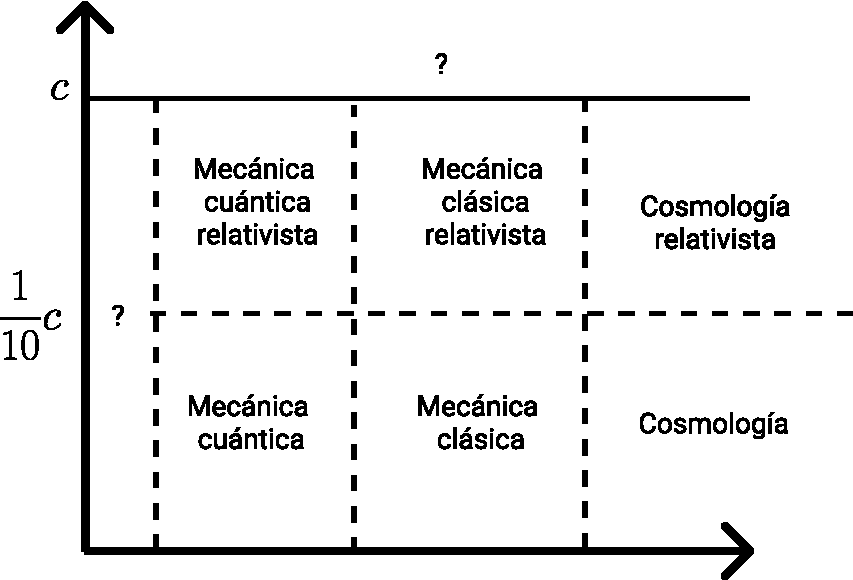
\includegraphics[width=0.6\textwidth]{es1.pdf}
	\caption{clasificación de la Mecánica}
\end{figure}

Se llama Mecánica Clásica, la Mecánica basada en las tres leyes de Newton. Actualmente la
Mecánica Clásica es todo un conjunto de asignaturas técnicas, generales y especiales, dedicadas a
la investigación del movimiento de los cuerpos sueltos y de sus sistemas, al análisis y diseño de
distintas obras de ingeniería, especialmente estructuras, máquinas y procesos. Dependiendo de la
naturaleza de los problemas que se examinan, la Mecánica Clásica se divide en:

\Schema{-1.4ex}{16ex}{\schemabox{Mecánica Clásica}}{\Schema{-1ex}{6ex}
	{\schemabox{De cuerpos Rígidos}}
	{{\schemabox{Estática}}\medskip\schema{\schemabox{Dinámica}}{\schemabox{Cinemática\\ Cinética}}}
	\Schema{-1ex}{2ex}
	{\schemabox{De cuerpos deformables}}{\schemabox{Mecánica de materiales\\Teoría de la elasticidad}}
	\Schema{-1ex}{2ex}
	{\schemabox{De fluidos}}{\schemabox{Incomprensibles (hidráulica)\\Comprensibles (Neumática)}}}

El objetivo de la Estática, como ciencia, es el estudio de las propiedades generales de las fuerzas
(como magnitudes físicas vectoriales) y las condiciones de equilibrio de los cuerpos sometidos
a la acción de fuerzas.

Problemas generales de la Estática como ciencia.

\begin{enumerate}
	\item Establecer los métodos para la composición y descomposición de fuerzas y la reducción
	      de los sistemas de fuerzas, aplicadas a un cuerpo, a su expresión más simple. Esto con el
	      propósito de predecir los efectos externos de las fuerzas sobre los cuerpos o sistemas.
	\item Determinar las condiciones de equilibrio de los cuerpos, sometidos a la acción de
	      sistemas de fuerzas, y su aplicación al análisis y diseño de sistemas de ingeniería,
	      principalmente máquinas y estructuras en general.
\end{enumerate}

Se convertirá la distancia $r$ de milímetros a metros

\begin{equation*}
	800mm=800mm \left(\frac{1m}{1,000mm}\right)=0.8m
\end{equation*}



\begin{problem}
La torre se mantiene en su lugar mediante tres cables. Si se muestra la fuerza de cada cable que actúa sobre la torre, determine la magnitud y los ángulos de dirección de coordenadas $\alpha, \beta, \gamma$ de la fuerza resultante. Tome $x = 15 m$, $y = 20 m$
\end{problem}

\begin{figure}[h!]
	\centering
	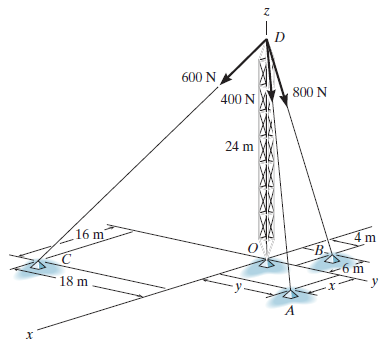
\includegraphics[width=0.5\textwidth]{es2.png}
	\caption{Problema 2-96}
	\label{es2png}
\end{figure}

\textit{ Sol. }

El problema busca resolver la magnitud y los ángulos de dirección de las coordenadas en ciertos ángulos que involucran a la fuerza resultante, por lo que la información que da el problema es la siguiente:

\begin{align*}
	 & F_R=?                           &  & \alpha=?                       &  & \beta=?                         &  & \gamma=? \\
	 & \cos\alpha=\frac{F_{Rx}}{F_{R}} &  & \cos\beta=\frac{F_{Ry}}{F_{R}} &  & \cos\gamma=\frac{F_{Rz}}{F_{R}} &  &
\end{align*}

Teniendo en cuenta los tres planos vectoriales, se definen las coordenadas en función de las distancias, siendo el centro del poste (el punto $O$) la coordenada $(0,0,0)$.

\begin{align*}
	 & A=(20,15,0) &  & B=(-6,4,0) &  & C=(16,-18,0) &  & D=(0,0,24)
\end{align*}

\begin{notation}
	Se puede representar con magnitud y sentido, a las fuerzas que están interactuando estáticamente:

	\begin{align*}
		 & \overrightarrow{r}_A=20\hat{i}+15\hat{j}m
		 &                                           & \overrightarrow{r}_B=-6\hat{i}+4\hat{j}m
		 &                                           & \overrightarrow{r}_C=16\hat{i}-18\hat{j}m
		 &                                           & \overrightarrow{r}_D=24\hat{k}m
	\end{align*}
\end{notation}



Todas las fuerzas son directamente de $D$ a los puntos $A,B,C$, por lo que se necesitan los valores de $\overrightarrow{r_{A/D}},\overrightarrow{r_{B/D}},\overrightarrow{r_{C/D}}$:

\begin{align*}
	 & \overrightarrow{r}_{A/D}=\overrightarrow{r}_A-\overrightarrow{r}_{D}=20i+15j24\hat{k}              &  & \left\lvert \overrightarrow{r}_{A/D} \right\rvert=34.66m \\
	 & \overrightarrow{r}_{B/D}=\overrightarrow{r}_B-\overrightarrow{r}_{D}=-6\hat{i}+4\hat{j}-24\hat{k}  &  & \left\lvert \overrightarrow{r}_{B/D} \right\rvert=25.06m \\
	 & \overrightarrow{r}_{C/D}=\overrightarrow{r_C}-\overrightarrow{r}_{D}=16\hat{i}-18\hat{j}-24\hat{k} &  & \left\lvert \overrightarrow{r}_{C/D} \right\rvert=34.00m
\end{align*}

Realizando los cocientes, expresamos:

\begin{align*}
	U_{A/D}=\frac{\overrightarrow{r}_{A/D}}{\left\lvert \overrightarrow{r}_{A/D} \right\rvert} &  & U_{B/D}=\frac{\overrightarrow{r}_{B/D}}{\left\lvert \overrightarrow{r}_{B/D} \right\rvert} &  & U_{C/D}=\frac{\overrightarrow{r}_{C/D}}{\left\lvert \overrightarrow{r}_{C/D} \right\rvert}
\end{align*}

Existen tres fuerzas sí y sólo sí hay tres cables, la notación a usar para las fuerzas equivalentes de dos, será $F_{ab}$:

\begin{align*}
	 & \overrightarrow{F}_{AD}=400\overrightarrow{U}_{A/D}=400\left(\frac{20}{34.66}\hat{i}+\frac{51}{34.66}\hat{j}-\frac{24}{34.66}\hat{k}\right)N \\
	 & \overrightarrow{F}_{BD}=400\overrightarrow{U}_{B/D}=800\left(\frac{-6}{25.06}\hat{i}+\frac{4}{25.06}\hat{j}-\frac{24}{25.06}\hat{k}\right)N  \\
	 & \overrightarrow{F}_{CD}=400\overrightarrow{U}_{C/D}=600\left(\frac{16}{34.66}\hat{i}-\frac{18}{34.66}\hat{j}-\frac{24}{34.66}\hat{k}\right)N
\end{align*}

Finalmente, la fuerza resultante, es producto de la suma de las tres fuerzas obtenidas anteriormente, cumpliendo con el equilibrio:

\begin{equation}
	F_R=F_{AD}+F_{BD}+F_{CD}
\end{equation}

\begin{align*}
	 & \overrightarrow{F_R}=321.66\hat{i}-16.82\hat{j}-14466.71\hat{k}N \\
	 & \left\lvert \overrightarrow{F}_R \right\rvert=1501.66N
\end{align*}

\begin{align*}
	 & \alpha=\arccos{\left(\frac{F_{Rx}}{\left\lvert F_R\right\rvert}\right)}=\arccos{\left(\frac{321.66}{1501.66}\right)} \\&\beta=\arccos{\left(\frac{F_{Ry}}{\left\lvert F_R\right\rvert}\right)}=\arccos{\left(\frac{-16.82}{1501.66}\right)}\\&\gamma=\arccos{\left(\frac{F_{R2}}{\left\lvert F_R\right\rvert}\right)}=\arccos{\left(\frac{-1466.71}{1501.66}\right)}
\end{align*}

Respuestas finales:

\begin{align*}
	 & F_R=1501.66N &  & \alpha=77.6^{\circ} &  & \beta=90.6^{\circ}N &  & \gamma=168.2^{\circ}N
\end{align*}


\section{Producto punto}

\begin{figure}[h!]
	\centering
	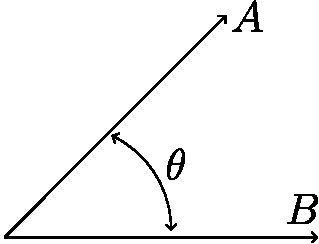
\includegraphics[scale=0.5]{es4.pdf}
	\caption{El ángulo formado de vectores}
	\label{es4pdf}
\end{figure}

Donde para calcular el ángulo se despeja de la ecuación \ref{productopunto}

\begin{equation}
	A\cdot B=AB\cos\theta
	\label{productopunto}
\end{equation}

como sigue:

\begin{align*}
	 & \theta=\arccos \left(\frac{A\cdot B}{AB}\right) &  & 0^{\circ}\leq\theta \leq 180^{\circ}
\end{align*}

Existen tres leyes de operación

\begin{align}
	 & \text{Conmutativa } A\cdot B=B\cdot A                      \\
	 & \text{Multiplicación } a(A\cdot B)= (aA)\cdot B=A\cdot(aB) \\
	 & \text{Distributiva } A\cdot (B+D)=(A\cdot B)+(A\cdot D)
\end{align}

\subsection{Formulación del vector cartesiano}

\begin{equation}
	i\cdot i=(1)(1)\cos 0^{\circ}=1\land i\cdot j=(1)(1)\cos 90^{\circ}=0
\end{equation}

La componente de un vector paralelo y perpendicular

\begin{align}
	 & A=A_a+A_{\perp}                                  \\
	 & A_a=A\cos(\theta)=A_a u_a                        \\
	 & \theta=\arccos \left(\frac{A\cdot u_A}{A}\right) \\
	 & A_{\perp}=A\sin(\theta)                          \\
	 & A_{\perp}=\sqrt{A^2-A^2_a}
\end{align}

\section{Compilación de problemas}

En matemática y física, un \textbf{vector}, es un ente matemático como la recta
o el plano. Un vector se representa mediante un segmento de recta, orientado
dentro del espacio euclidiano tridimensional. El vector tiene 3 elementos:
módulo, dirección y sentido. Los vectores nos permiten representar magnitudes
físicas vectoriales, como las mencionadas líneas abajo.

\begin{problem}
Exprese la fuerza F como un vector cartesiano; después, determine sus ángulos directores coordenados.
\end{problem}

\begin{figure}[h!]
	\centering
	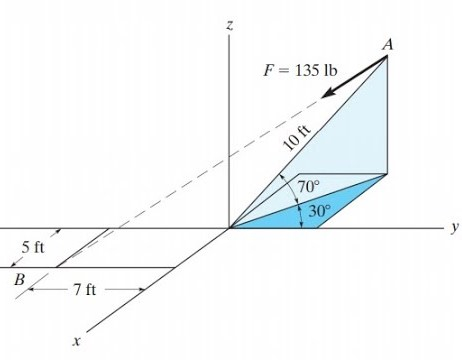
\includegraphics[width=0.5\textwidth]{es5.jpg}
	\caption{Problema 2-87.}
	\label{es5pdf}
\end{figure}

\textit{ Sol.}

\begin{align*}
	 & r_{AB}=r_B-r_A                                                                     \\
	 & r_{AB}=(X_B-x_A)i+(Y_B-Y_A)j+(Z_B-z_a)k                                            \\
	 & r_{AB}=((5)-(-1.71))i+((-7)-(2.96)j+(10)-(9.4)k                                    \\
	 & r_{AB}=6.71i-9.96j-9.4k                                                            \\
	 & \mid r_{AB}=\sqrt{6.71^2+9.96^2+9.4^2}=15.25                                       \\
	 & F_{AB}=FU_{AB}=F\left(\frac{r_{AB}}{r_{AB}} \right)                                \\
	 & F_{AB}=135\left(\frac{6.71i}{15.25}-\frac{9.96j}{15.25}-\frac{9.4k}{15.25} \right) \\
	 & F_{AB}=59.4i-88.17j-83.2k                                                          \\
	 & \alpha=\arccos\left(\frac{6.71}{15.25} \right))63.9^{\circ}                        \\
	 & \beta=\arccos\left(\frac{-9.96}{15.25} \right))63.9^{\circ}                        \\
	 & \gamma=\arccos\left(\frac{-9.4}{15.25} \right))63.9^{\circ}
\end{align*}

Por lo que los resultados finales son:

\begin{align*}
	 & F_{AB}=59.4i-88.17j-83.2k                                   \\
	 & \alpha=\arccos\left(\frac{6.71}{15.25} \right))63.9^{\circ} \\
	 & \beta=\arccos\left(\frac{-9.96}{15.25} \right))63.9^{\circ} \\
	 & \gamma=\arccos\left(\frac{-9.4}{15.25} \right))63.9^{\circ}
\end{align*}

%%%%%%%%%%%%%%%%%%%%%%%%%%%%%%%%%%%%%%%%%%%%%%%%%%%%%%%%%%%%%%%%%%%%%%%%%%%%%%%%%%%%%%%%%%%%%%%%

\begin{problem}
Si $F=350i - 250j - 450k N $y el cable $AB$ tiene $9m$ de longitud, determine las coordenadas $x, y, z$ del punto $A$.
\end{problem}

\begin{figure}[h!]
	\centering
	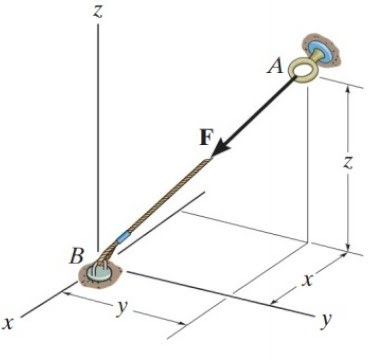
\includegraphics[width=0.5\textwidth]{es6.jpg}
	\caption{Problema 2-89.}
	\label{es6pdf}
\end{figure}

\textit{ Sol.}

\begin{align*}
	 & F=350i-250j-450k                                               \\
	 & \mid F\mid=\sqrt{350^2+250^2+450^2}=622.5                      \\
	 & \alpha=\arccos\left(\frac{350}{622.5}\right)=55.78^{\circ}     \\
	 & \beta=\arccos\left( \frac{-250}{622.5} \right)=136.67^{\circ}  \\
	 & \gamma=\arccos \left( \frac{-450}{622.5}\right)=136.29^{\circ}
\end{align*}

\begin{align*}
	 & A_x=\mid A\mid \cos \alpha                             \\
	 & A_x=\mid A\mid \cos 55.78^{\circ}=5.06m                \\
	 & A_y=\mid A\mid \cos B=9\cos (113.67^{\circ})=3.61m     \\
	 & A_z=\mid A\mid\cos \gamma =9\cos (136.29^{\circ})=6.5m \\
	 & A=(-5.06,3.61,6.5)
\end{align*}

Respuesta final:

\begin{equation*}
	A=(-5.06,3.61,6.5)
\end{equation*}

%%%%%%%%%%%%%%%%%%%%%%%%%%%%%%%%%%%%%%%%%%%%%%

\begin{problem}
Si $FB=700 N$ y $FC 560 N$, determine la magnitud y los ángulos directores coordenados de la fuerza resultante que actúa sobre el asta de la bandera.
\end{problem}

\begin{figure}[h!]
	\centering
	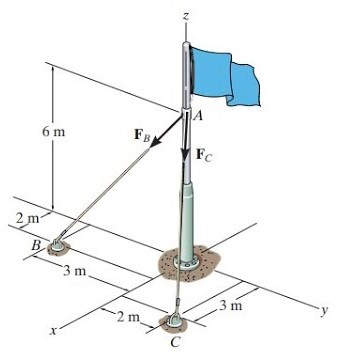
\includegraphics[width=0.5\textwidth]{es7.jpg}
	\caption{Problema 2-93/94.}
	\label{es7}
\end{figure}


\textit{ Sol.}

\begin{align*}
	 & U_B=\frac{r}{\mid r\mid}\implies \mid r\mid=\sqrt{2^2+(-3)^2+(-6)^2}=7                        \\
	 & r_B=2i-3j-6k                                                                                  \\
	 & F_B=FU_B=700\left( \frac{2i}{7}-\frac{3j}{7}-\frac{6k}{7} \right)                             \\
	 & F_B=200i-300j-600k                                                                            \\
	 & r_C=3i+2j-6k\implies U_C=\frac{r_C}{\mid r_C \mid}\implies \mid r_C \mid=\sqrt{3^2+2^2+6^2}=7 \\
	 & F_C=FU_C=560\left( \frac{3i}{7}+\frac{2j}{7}-\frac{6k}{7} \right)                             \\
	 & F_C=240i+160j-480k                                                                            \\
	 & F_R=F_B+F_C=440i-140j-1080k                                                                   \\
	 & \mid F_R \mid=\sqrt{490^2+140^2+1080^2}=1174.56
\end{align*}

Respuesta final:

\begin{align*}
	 & \mid F_R \mid= 1174.56                                                      \\
	 & \alpha=\arccos \left( \frac{440}{1174.56} \right)=68^{\circ}                \\
	 & \beta=\arccos \left( \frac{-140}{1174.56} \right)=96.84^{\circ}             \\
	 & \gamma= \arccos \arccos \left( \frac{-1080}{1174.56} \right)=156.85^{\circ} \\
\end{align*}

%%%%%%%%%%%%%%%%%%%%%%%%%%%%%%%%%%%%%%%%%%%%%%

\begin{problem}
La placa se encuentra suspendida de tres cables que ejercen las fuerzas mostradas en la figura \ref{es8pdf}. Exprese cada fuerza como un vector cartesiano.
\end{problem}

\begin{figure}[h!]
	\centering
	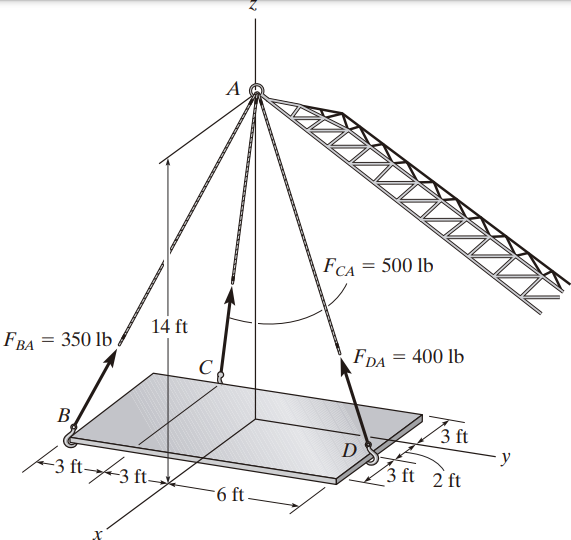
\includegraphics[width=0.5\textwidth]{es8.png}
	\caption{Problema 2-95.}
	\label{es8pdf}
\end{figure}

\textit{ Sol.}

\begin{align*}
	 & r_{BA}=-5i+6j+14k\implies \mid r_{BA} \mid=\sqrt{5^2+6^2+4^2}=16.03                                                                  \\
	 & F_{BA}=FU_{BA}=F\left( \frac{r_{BA}}{\mid r_{BA} \mid} \right)=350\left( \frac{-5i}{16.03}+\frac{6j}{16.03}+\frac{14k}{16.03}\right) \\
	 & \implies F_{BA}=-109.17i+131.004j+305.67k                                                                                            \\
\end{align*}

\begin{align*}
	 & r_{CA}=3u+3j+14k\implies \mid r_{CA}\mid =\sqrt{3^2+3^2+14^2}=14.62          \\
	 & F_{CA}=500\left( \frac{3i}{14.62}+\frac{3j}{14.62}+\frac{14k}{14.62} \right) \\
	 & F_{CA}=103i+103j+479k
\end{align*}

\begin{align*}
	 & r_{DA}=-2i-6j+14k\implies \mid r_{DA}=\sqrt{2^2+6^2+14^2}=15.36               \\
	 & F_{DA}=400\left(\frac{-2i}{15.36}-\frac{-6j}{15.36}+\frac{14k}{15.36} \right) \\
	 & F_{DA}=-52.1i-156.25j+365k
\end{align*}

%%%%%%%%%%%%%%%%%%%%%%%%%%%%%%%%%%%%%%%%%%%%%%

\begin{problem}
Los dos cables de amarre ejercen fuerzas sobre la popa de un barco, como se muestra en la figura. Represente cada fuerza como un vector cartesiano; además, determine la magnitud y los ángulos directores coordenados de la resultante.
\end{problem}

\begin{figure}[h!]
	\centering
	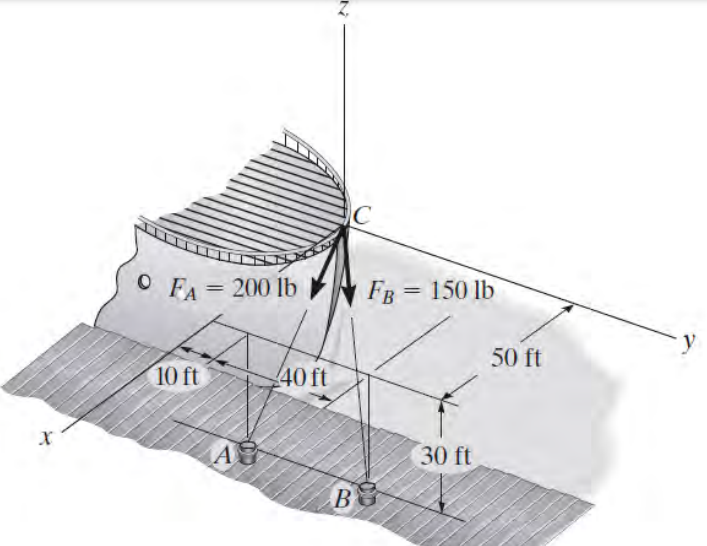
\includegraphics[width=0.5\textwidth]{es9.png}
	\caption{Problema 2-101.}
	\label{es9png}
\end{figure}

\textit{ Sol.}

\begin{align*}
	 & r_{CA}=50i+10j-30k\implies \mid r_{CA}=\sqrt{50^2+10^2+30^2}=59.16            \\
	 & r_{CA}=200\left(\frac{50i}{59.16}+\frac{10j}{59.16}-\frac{30k}{59.16} \right) \\
	 & F_{CA}=169i+33.8j-101.4klb
\end{align*}

\begin{align*}
	 & r_{CB}=50i+50j-30k\implies \mid r_{CB}=\sqrt{50^2+50^2+30^2}=76.81        \\
	 & F_{CB}=150\left(\frac{50i}{76.8}+\frac{50j}{76.8}-\frac{30k}{76.8}\right) \\
	 & F_{CA}=169i+33.8j-101.4k\quad lb
\end{align*}

\begin{align*}
	 & F_R=2.66.6i+131.4j3160k                             \\
	 & \mid F_R\mid =\sqrt{266.6^2+131.4^2+160^2}=337.55lb
\end{align*}

\begin{align*}
	 & \alpha=\arccos \left(\frac{266.6}{337.55}\right)=37.83^{\circ}  \\
	 & \beta=\arccos \left(\frac{131.4}{337.55} \right)=67.09^{\circ}  \\
	 & \gamma=\arccos \left(\frac{-160}{337.55} \right)=118.29^{\circ}
\end{align*}

%%%%%%%%%%%%%%%%%%%%%%%%%%%%%%%%%%%%%%%%%%%%%%

\begin{problem}
Determine la magnitud y los ángulos directores coordenados de la fuerza resultante.
\end{problem}

\begin{figure}[h!]
	\centering
	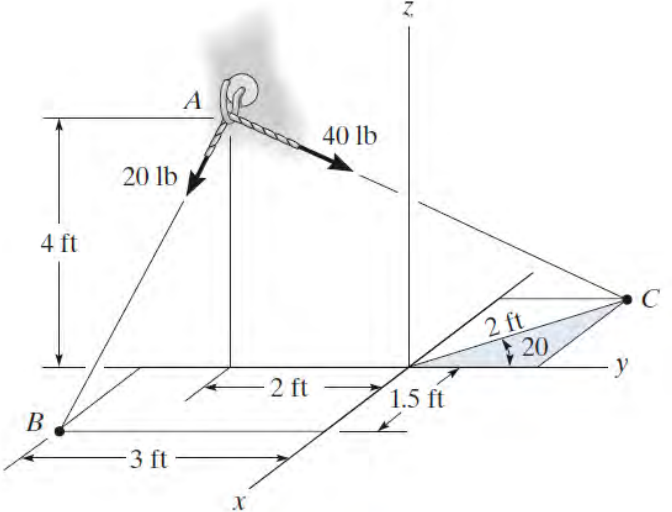
\includegraphics[width=0.5\textwidth]{es10.png}
	\caption{Problema 2-103.}
	\label{es10}
\end{figure}

\textit{ Sol.}

\begin{align*}
	 & r_{AB}=(x_B-x_A)i+(y_B-y_A)j+(2_B-z_A)k    \\
	 & r_{AB}=(1.5-0)i+(-3-(-2))j+(0-4)k          \\
	 & r_{AB}=1.5i-1-4k                           \\
	 & \mid r_{AB}\mid =\sqrt{1.5^2+1^2+4^2}=4.38 \\
\end{align*}

\begin{align*}
	 & F_{AB}=6.85i-4.56j-18.26k                                                       \\
	 & r_{AC}=(-0.68-0)i+(1.88-(-2))j+(0-4)k                                           \\
	 & r_{AC}=-0.68i+3.88j-4k\implies \mid r_{AC}=\sqrt{0.68^2+3.88^2+4^2}=5.61        \\
	 & F_{AC}=40\left( \frac{-0.68i}{5.61}+\frac{3.88j}{5.61}-\frac{4k}{5.610} \right)
\end{align*}

\begin{align*}
	 & F_{AC}=-4.84i+27.7j-28.52k                  \\
	 & F_R=2.01i+23.14j-46.78k                     \\
	 & \mid F_R\mid =\sqrt{2.01^2+23.14^2+46.78^2} \\
	 & \mid F_R\mid =52.2lb
\end{align*}

\begin{align*}
	 & \alpha=\arccos \left( \frac{2.01}{52.2}\right)=87.8^{\circ}    \\
	 & \beta=\arccos \left(\frac{23.14}{52.2}\right)=63.68^{\circ}    \\
	 & \gamma=\arccos \left(\frac{-46.78}{52.2}\right)=153.66^{\circ}
\end{align*}

%%%%%%%%%%%%%%%%%%%%%%%%%%%%%%%%%%%%%%%%%%%%%%

\begin{problem}
Determine la magnitud de la proyección de la fuerza $F=600N$ a lo largo del eje $U$.
\end{problem}

\begin{figure}[h!]
	\centering
	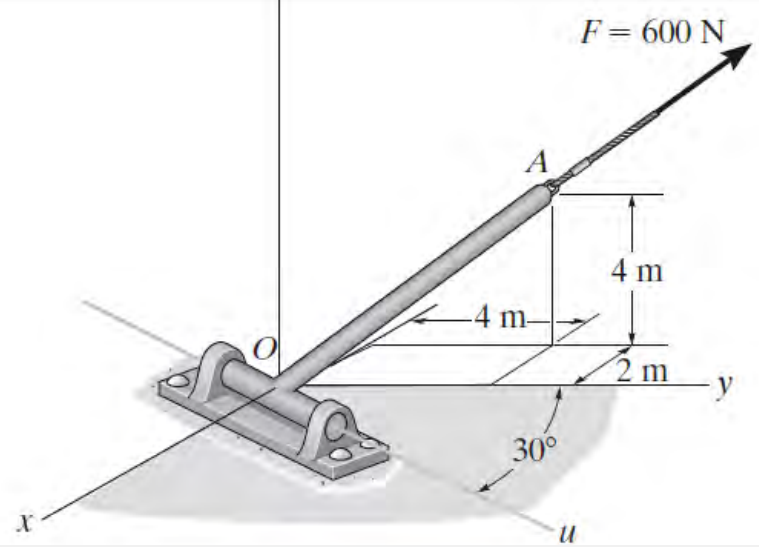
\includegraphics[width=0.5\textwidth]{es11.png}
	\caption{Problema 2-125.}
	\label{es11}
\end{figure}


\textit{ Sol. }

\begin{align*}
	 & W_A=-2i+4j+4k                                                                                               \\
	 & U=1\sin 30^{\circ}+1\cos 30^{\circ}j+10k                                                                    \\
	 & U=0.5i+0.966j+0k                                                                                            \\
	 & F_A=FU_A=600\left(\frac{r_A}{\mid r_A \mid}\right)=600\left(-\frac{2i}{6}+\frac{4j}{6}+\frac{4k}{6} \right) \\
	 & F_A=-200i+400j+400k                                                                                         \\
	 & \text{Proy. }F_{AU}=\left(-200i+400j+400k\right)\cdot \left( 0.5i+0.860j+0k \right)                         \\
	 & \text{Proy. }F_{AU}=-100+346.4+0=246.4
\end{align*}


\begin{problem}
Determine el ángulo entre los cables $AB$ y $AC$
\end{problem}

\begin{figure}[h!]
	\centering
	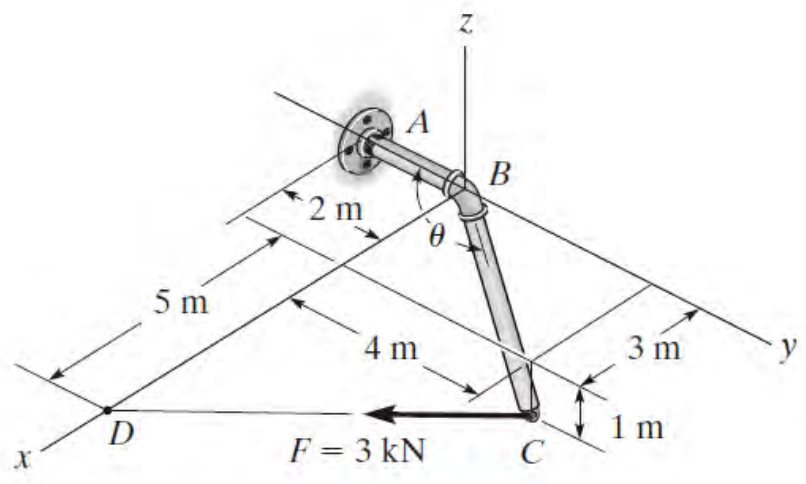
\includegraphics[width=0.5\textwidth]{es12.png}
	\caption{Problema 2-120/121}
	\label{es12}
\end{figure}

\textit{ Sol. }


\begin{align*}
	 & r_{AC}=\left(5\cos 60^{\circ}i+(0-6)j+(5\sin 60^{\circ}-2)k\right)                     \\
	 & \mid r_{AC}\mid=\sqrt{(5\cos 60)^2+6^2+2.33^2}=6.904                                   \\
	 & r_{AB}=-3i-6j+2k                                                                       \\
	 & r_{AB}=\sqrt{3^2+6^2+2^2}=7                                                            \\
	 & \theta=\arccos\left(\frac{r_{AC}\cdot r_{AB}}{\mid r_{AC}\mid \mid r_{AB}\mid }\right) \\
	 & r_{AC}\cdot r_{AB}=(2.5i-6j+2.33k)\cdot (-3i-6j+2k)=-7.5+36+4.66=33.16                 \\
	 & \theta=\arccos\left(\frac{33.16}{6.904\cdot 7}\right)=46.67
\end{align*}

\begin{problem}
Determine el ángulo entre los dos cables de la figura \ref{es13}
\end{problem}

\begin{figure}[h!]
	\centering
	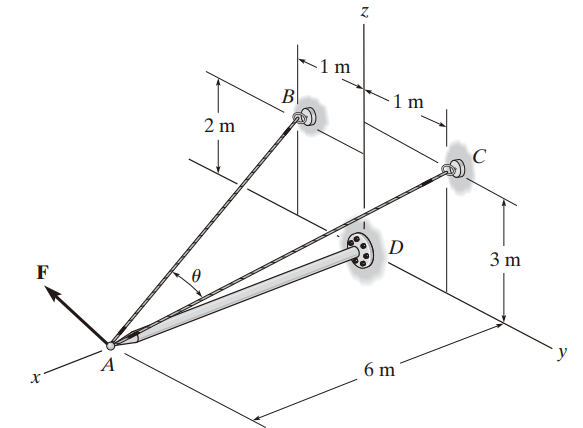
\includegraphics[width=0.5\textwidth]{es13.png}
	\caption{Problema 2-122/123}
	\label{es13}
\end{figure}


\textit{ Sol. }


\begin{align*}
	 & r_{AB}=(0-2)i+\left(3-(-3)\right)j+(0-3)k                                    \\
	 & r_{AB}=-2i+6j-3k                                                             \\
	 & \mid r_{AB}\mid =\sqrt{2^2+6^2+3^2}=7                                        \\
	 & r_{AC}=(-2-2)i+(3+3)j+(4-3)k                                                 \\
	 & r_{AC}=-4i+6j+1k                                                             \\
	 & \mid r_{AB}\mid =\sqrt{4^2+6^2+1^2}=7.28                                     \\
	 & \theta=\arccos\left(\frac{r_{AB}\cdot r_{AC}}{\mid r_{AB}\mid r_{AC}}\right) \\
	 & r_{AB}\cdot r_{AC}=(-2i+6j-3k)\cdot (-4i+6j+1k)=8+36-3=41                    \\
	 & \theta=\arccos\left(\frac{41}{7\cdot 7.28}\right)=36.43^{\circ}
\end{align*}


\begin{problem}
Determine la magnitud de la proyección de la fuerza $F_1$ a lo largo del cable $AC$
\end{problem}
\textit{ Sol. }

\begin{align*}
	 & F_1=FU_{AB}=F\left(\frac{r_{AB}}{r_{AB}}\right)=70\left(\frac{-2i}{7}+\frac{6j}{7}-\frac{3k}{7}\right)=-20i+60j-30k \\
	 & \text{Proy. } F_1(AC)=(-20i+60j-30k)\cdot (-0.55i+0.824j+0.137k)                                                    \\
	 & =11+49.44-4.11=56.33N
\end{align*}

\begin{problem}
Determine las magnitudes de los componentes de la fuerza $F=(60i+12j-40k)N$ proyectadas a lo largo de los cables $AB$ y $AC$
\end{problem}

\begin{figure}[h!]
	\centering
	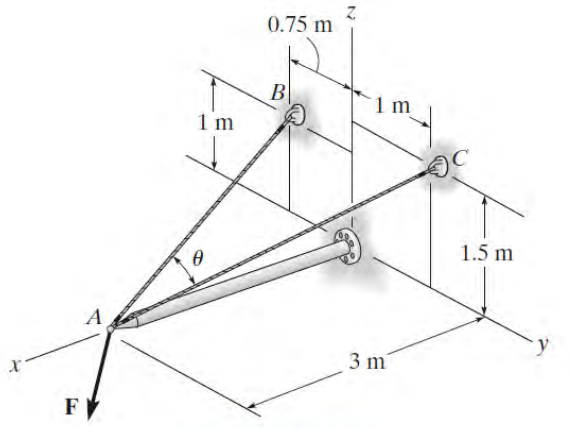
\includegraphics[width=0.5\textwidth]{es14.png}
	\caption{Problema 2-117/118}
	\label{es14}
\end{figure}

\textit{ Sol. }

\begin{align*}
	 & r_{AB}=(0-3)i+(-0.75-0)j+(1-0)k                                                                                    \\
	 & r_{AB}=-3i-0.75j+1k                                                                                                \\
	 & \mid r_{AB}\mid =\sqrt{3^2+0.75^2+1^2}=3.25                                                                        \\
	 & \text{Proy. } F_{AB}=F\cdot U_{AB}                                                                                 \\
	 & U_{AB}=\left(\frac{r_{AB}}{\mid r_{AB}\mid}\right)=\left(\frac{-3i}{3.25}-\frac{0.75}{3.25}+\frac{1k}{3.25}\right) \\
	 & U_{AB}=-0.923i-0.2307j+0.307k                                                                                      \\
	 & \text{Proy. }F_{AB}=(60i+12j-40k)(-0.923i-0.2307j+0.307k)=                                                         \\
	 & -55.38-2.7684-12.28                                                                                                \\
	 & \text{Proy. }F_{AB}=-70.4284N                                                                                      \\
	 & r_{AC}=(0-3)i+(1-0)j+(1.5-0)k\implies r_{AC}=-3i+1j+1.5k\implies                                                   \\
	 & \mid R_{AC}\mid =\sqrt{3^2+1^2+1.5^2}=3.5                                                                          \\
	 & U_{AC}=\left(\frac{-3i}{3.5}+\frac{1j}{3.5}+\frac{1.5}{3.5}\right)U_{AC}=-0.857i+0.2857j+0.4285k                   \\
	 & \text{Proy. }F_{AC}=F\cdot U_{AC}=(60i+12j-40k)\cdot(-0.857i+0.2857j+0.4285k)                                      \\
	 & \text{Proy. }F_{AC}=-51.42i+3.4284-17.14=-65.13N
\end{align*}


\begin{problem}
Si FB 36 lb y FC 45 lb, determine el momento resultante con respecto al perno ubicado en A.
\end{problem}

\begin{figure}[h!]
	\centering
	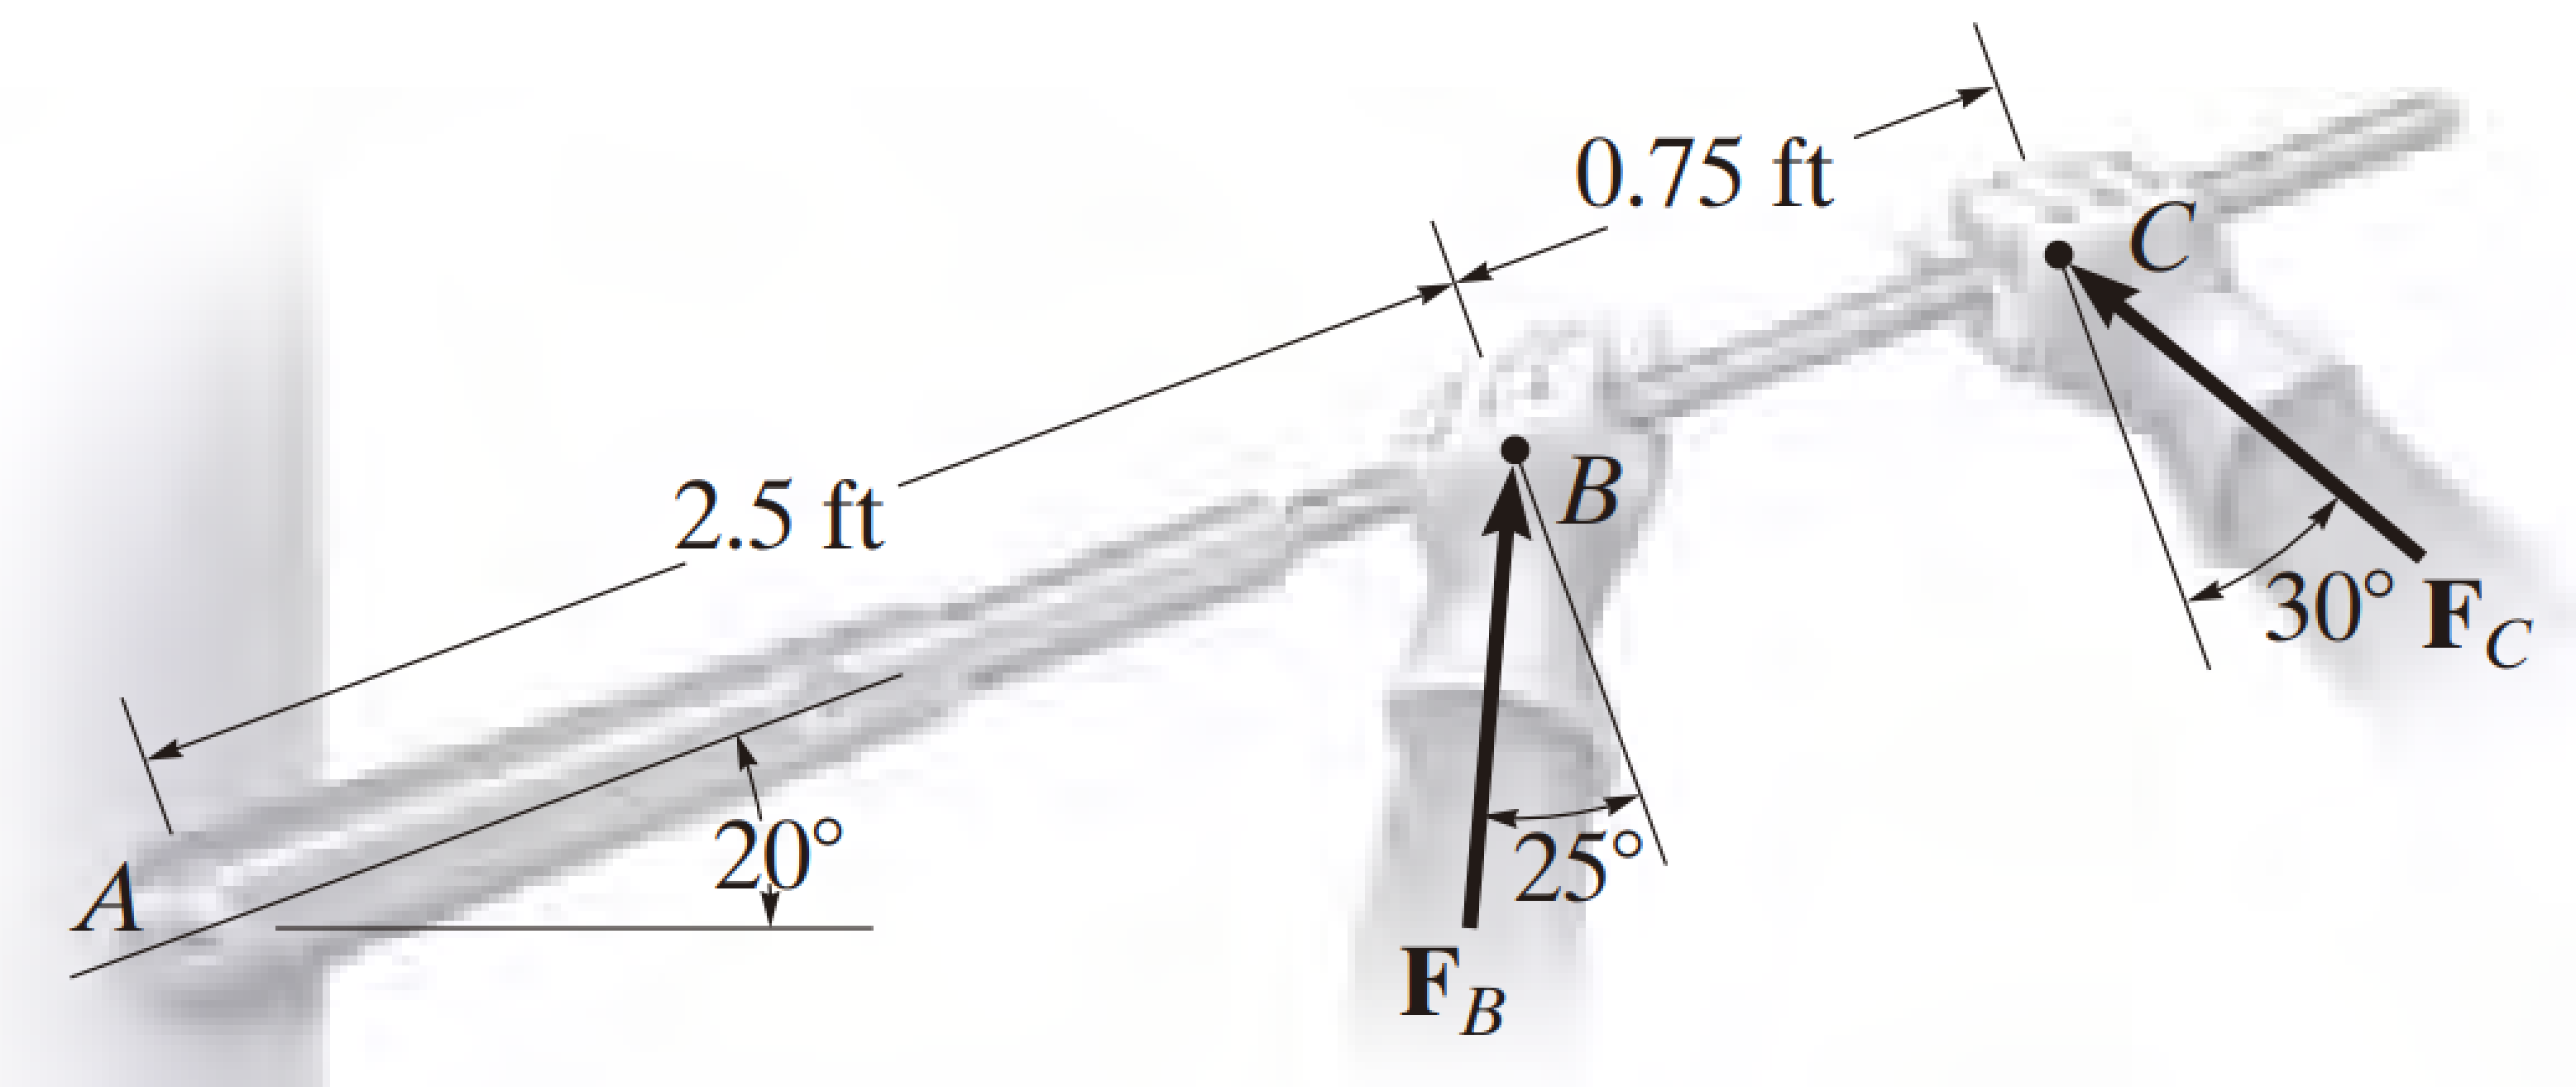
\includegraphics[scale=0.3]{es15.png}
	\caption{Problema 10}
\end{figure}

\textit{ Sol.}

\begin{align*}
	 & F_{BY}=36\sin{25^{\circ}}=15.2114 lb             \\
	 & F_{BX}=36\cos{25^{\circ}}=32.327 lb              \\
	 & M_B=(32.627)2.5081.5 lbft                        \\
	 & M_C=(45lb)(3.25\cdot \sin{60^{\circ}})=126.6lbft \\
	 & (M_R)_A=MB+M_C?81.5lbft+126.6lbft=208.1 lbft     \\
\end{align*}

Por lo tanto el momento resultante es: $208.1$ lbft


\begin{problem}
El cable ejerce una fuerza de $P=6 kN$ en el extremo del brazo de la grúa que tiene $8 m$ de longitud. Si $\theta=30^{\circ}$, determine la ubicación $x$ del gancho en $B$, de modo que esta fuerza cree un momento máximo con respecto al punto $O$. ¿Cuál es ese momento?
\end{problem}

\begin{figure}[h!]
	\centering
	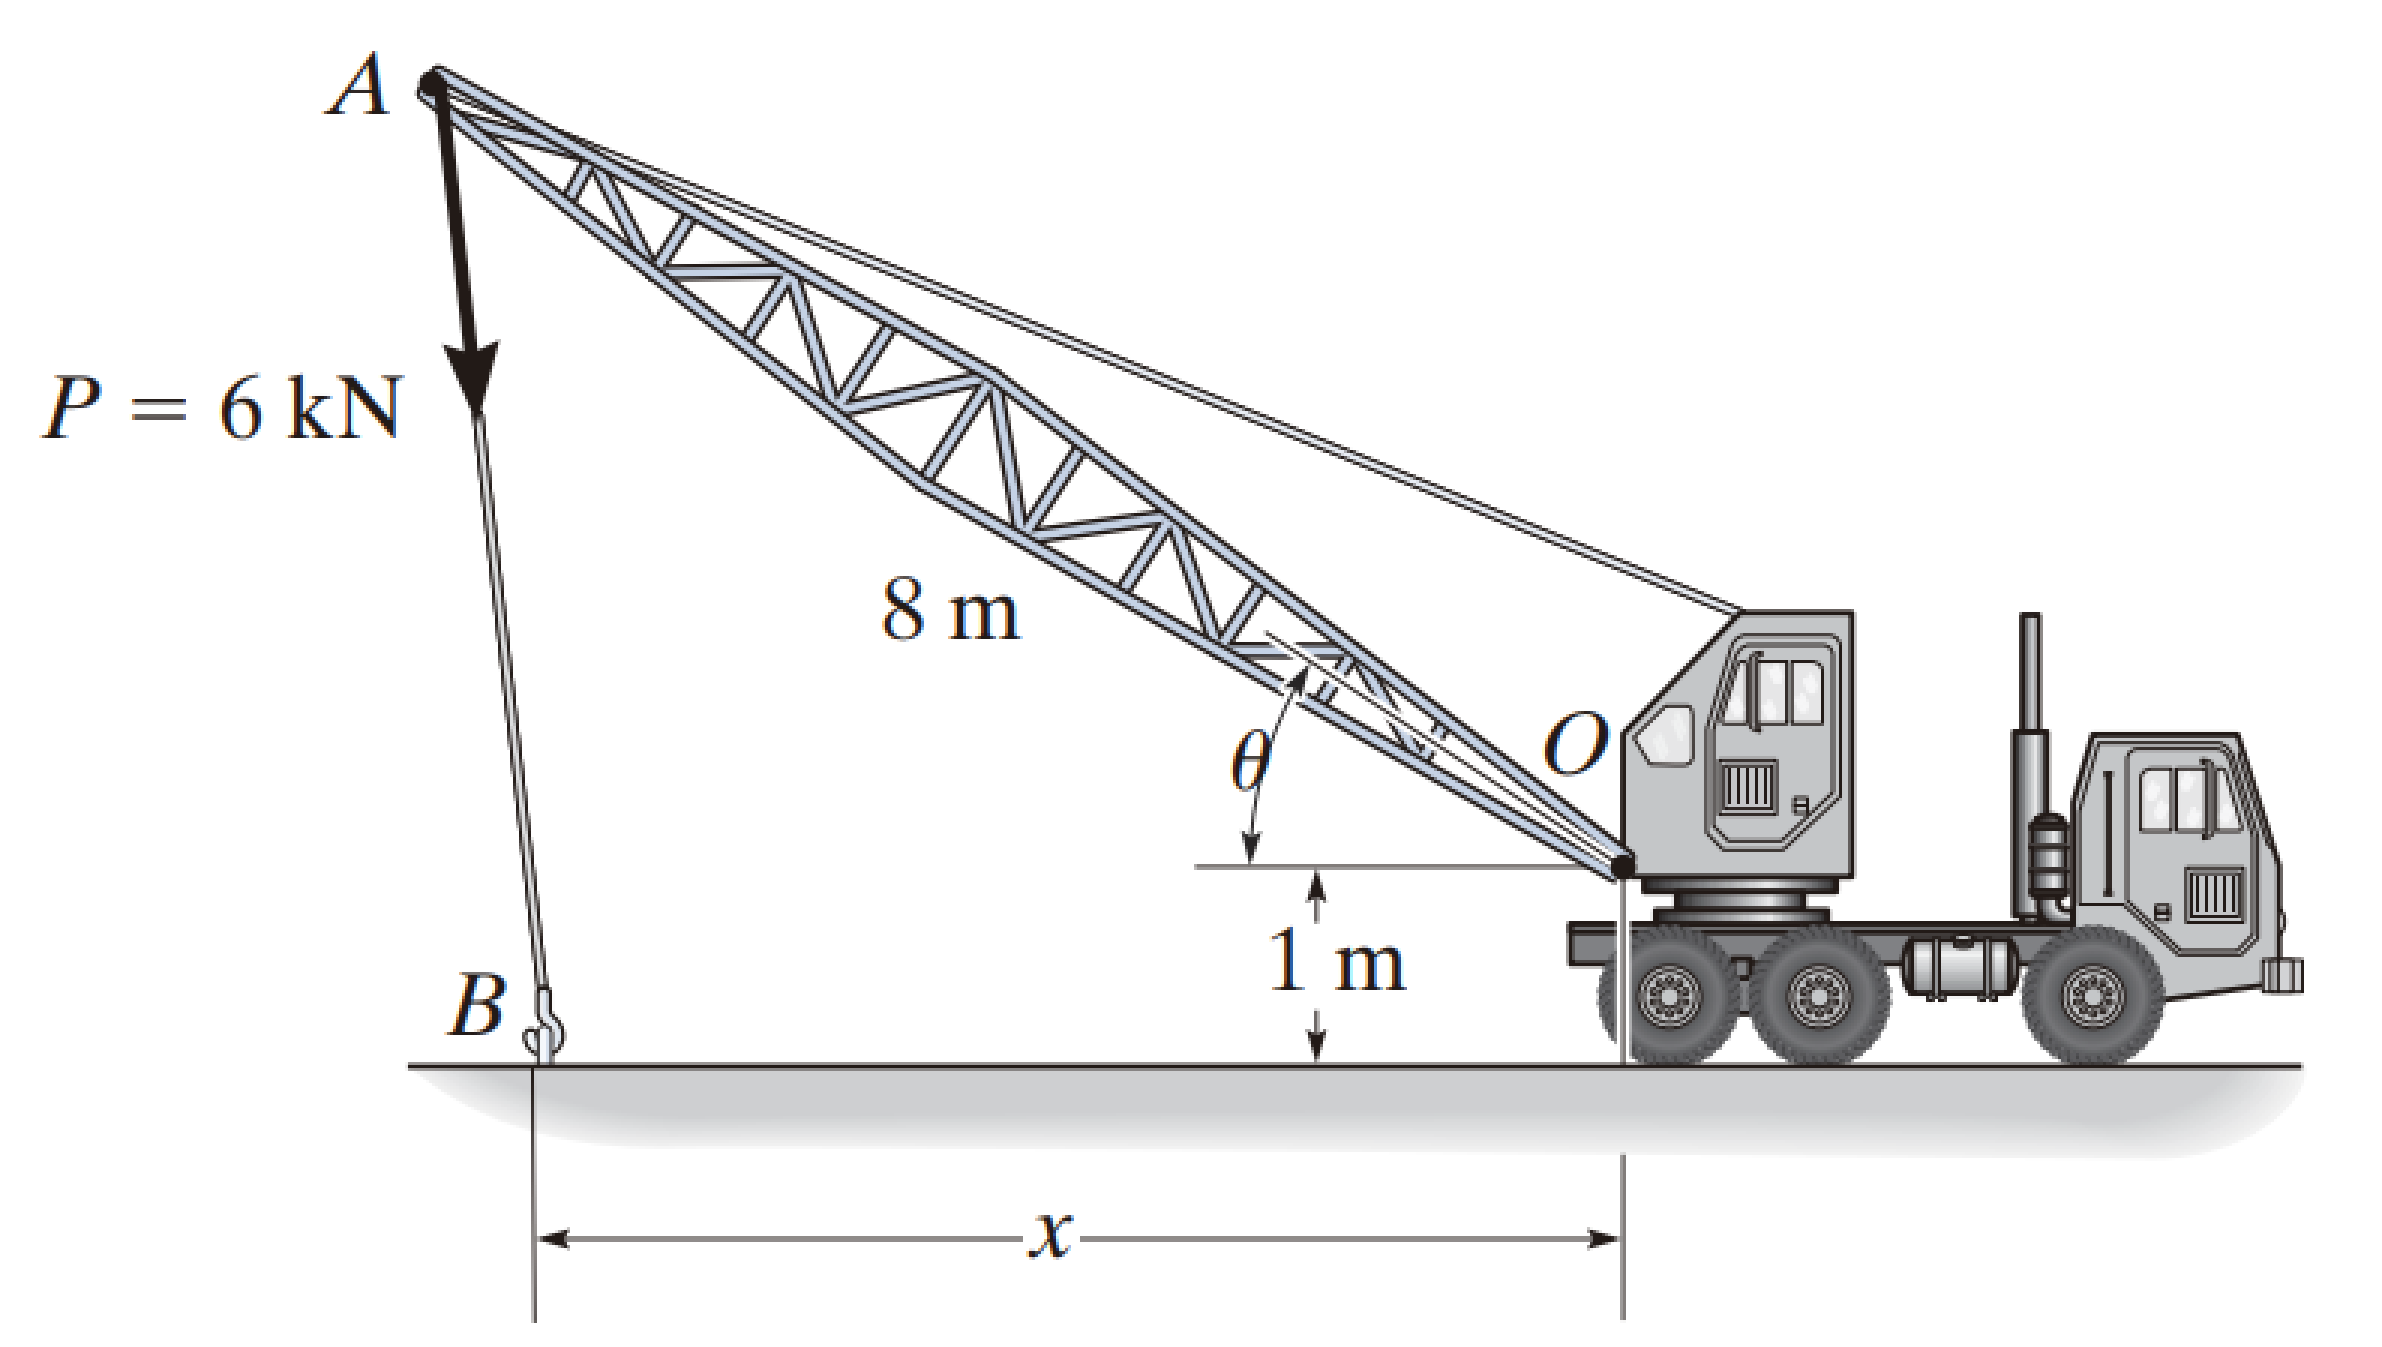
\includegraphics[scale=0.3]{es16.png}
	\caption{Problema 11}
\end{figure}

\textit{ Sol.}

Planteando el diagrama como un triángulo recto, tenemos las siguientes expresiones sabiendo que $M_0=F\cdot d$

\begin{align*}
	 & (M_0)_{Max}=6KN\cdot 8m=75KNm                            \\
	 & y=\frac{8}{\cos{30^{\circ}}}                             \\
	 & x=\frac{8}{\cos{30^{\circ}}}+\tan{30^{\circ}}=9.23+0.577 \\
	 & =9.8m
\end{align*}

El ángulo por buscar es: $\theta=31.53^{\circ}$


\begin{problem}
El cable ejerce una fuerza de $P=6 kN$ en el extremo del brazo de la grúa que tiene $8 m$ de longitud. Si $x=10 m$, determine la posición del brazo para que esta fuerza cree un momento máximo con respecto al punto $O$. ¿Cuál es ese momento?
\end{problem}

\begin{figure}[h!]
	\centering
	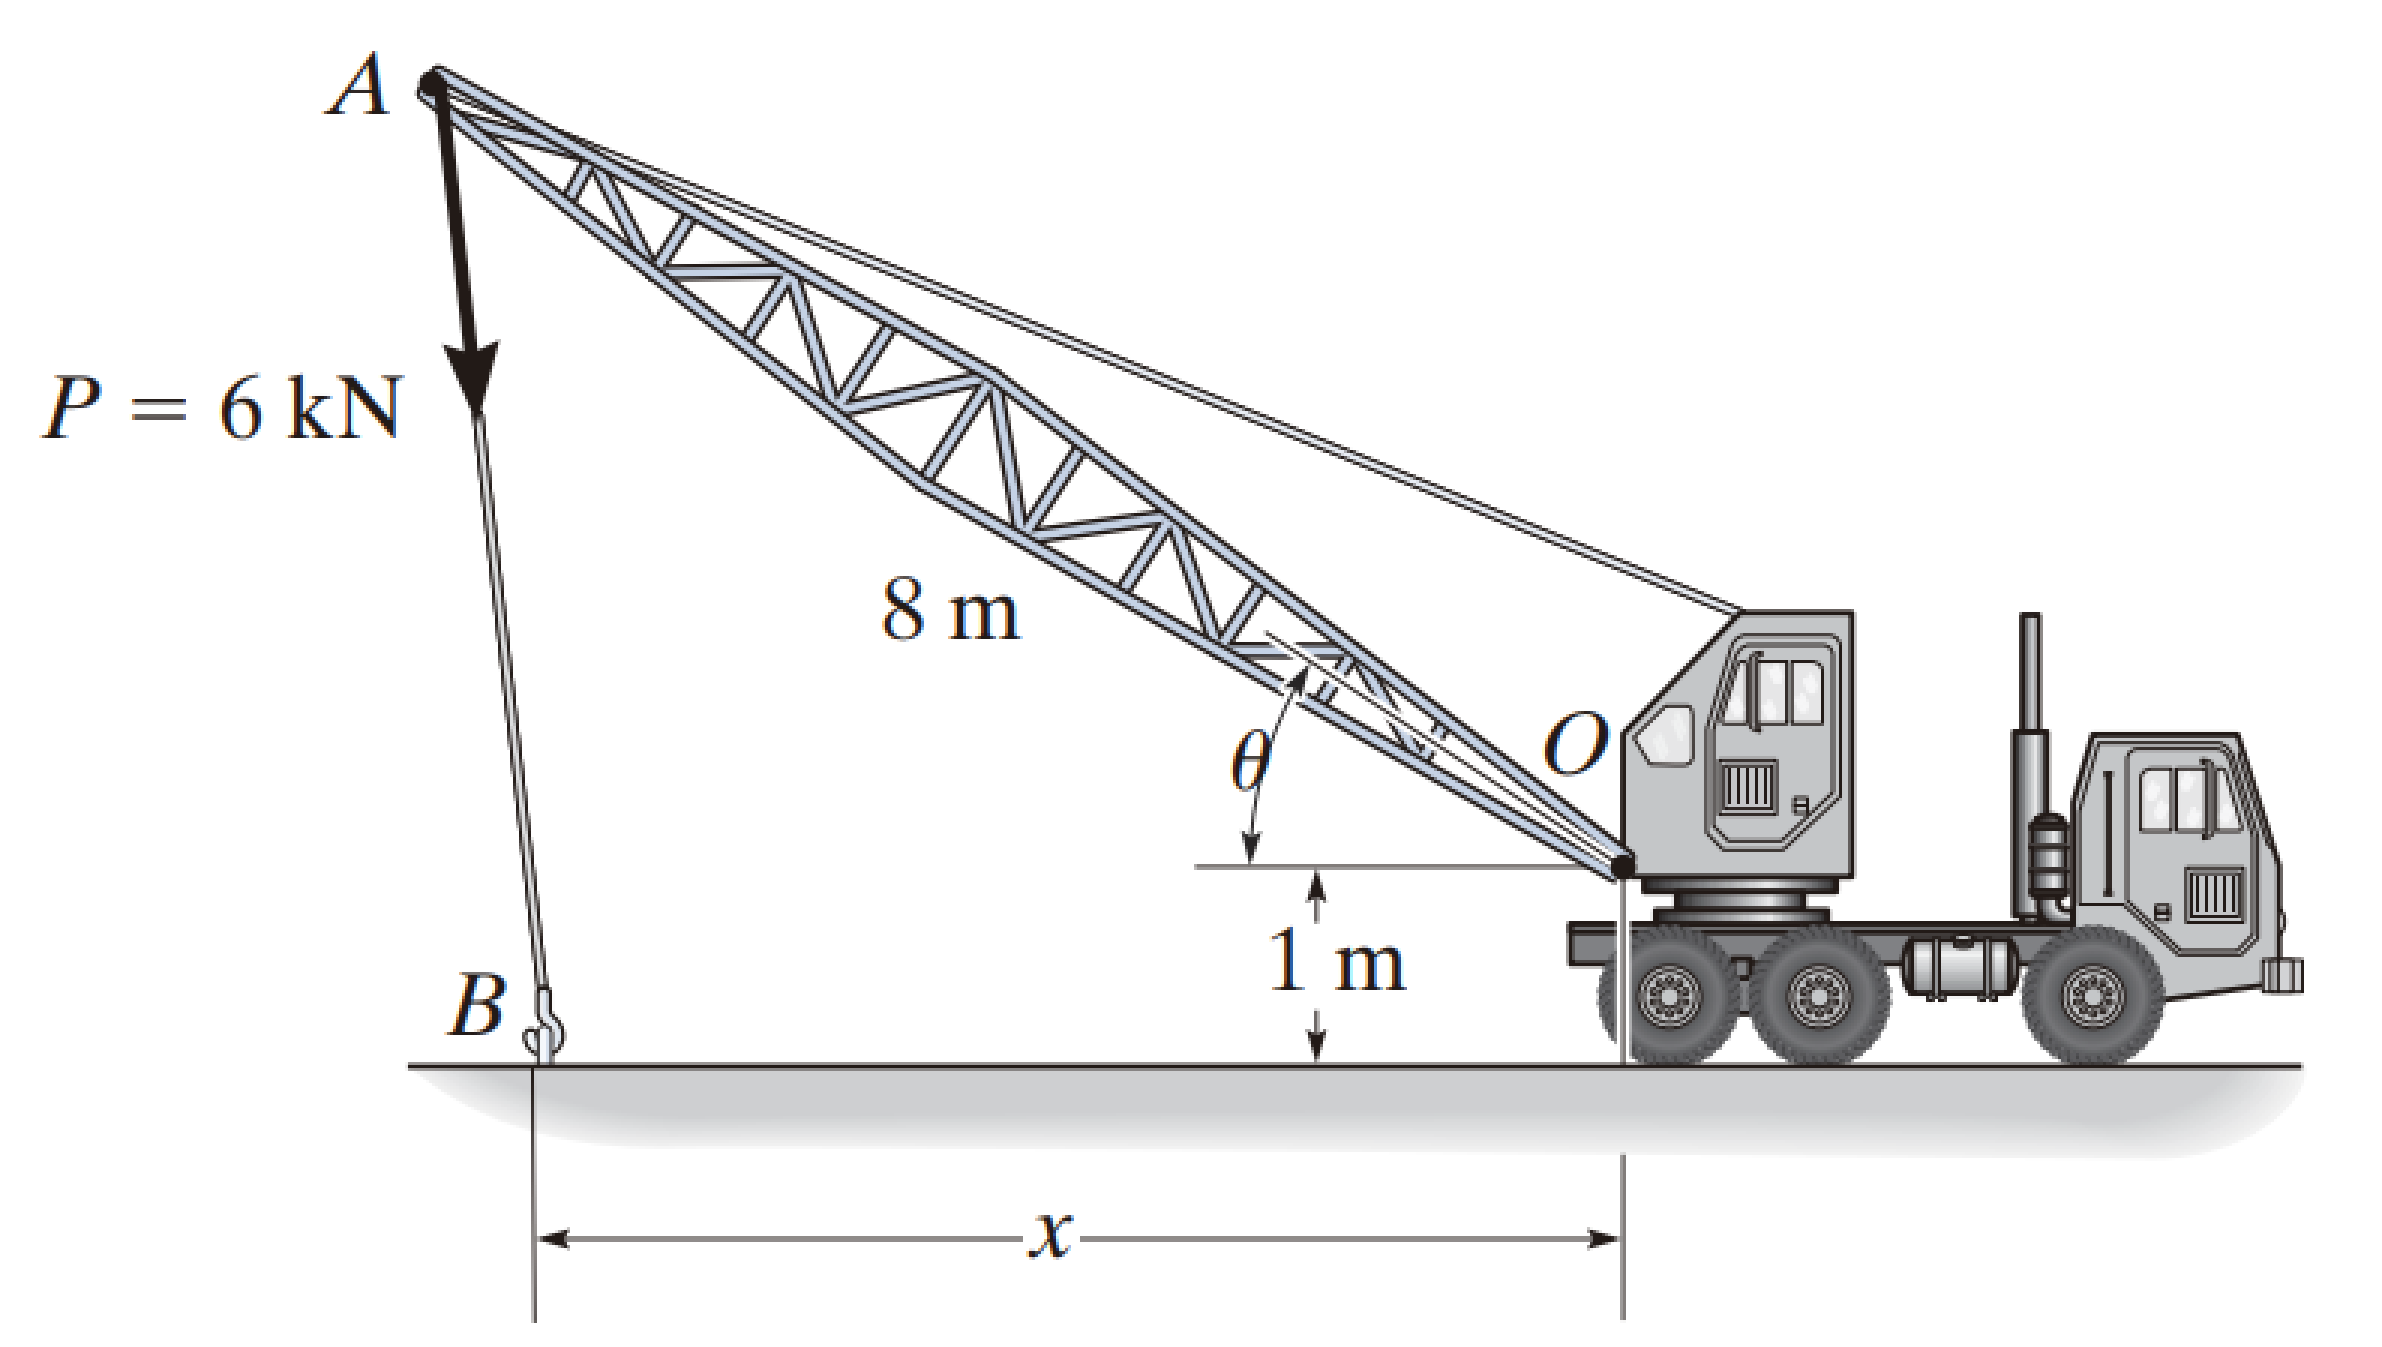
\includegraphics[scale=0.3]{es16.png}
	\caption{Problema 11}
\end{figure}

\textit{ Sol.}

\begin{align*}
	 & F_X=F\cdot \cos{30^{\circ}}                                  \\
	 & F_Y=F\cdot \sin{30^{\circ}}                                  \\
	 & M_A=-F\cdot \cos{30^{\circ}}\cdot-F\cdot \sin{30^{\circ}}(5) \\
	 & M_A=-20\cos{30^{\circ}}\cdot 18-20\sin{(30)5}                \\
	 & M_A=361.77lbin
\end{align*}



\begin{problem}
El mango del martillo está sometido a la fuerza de $F=20 lb.$ Determine el momento de esta fuerza con respecto al punto $A$.
\end{problem}

\begin{figure}[h!]
	\centering
	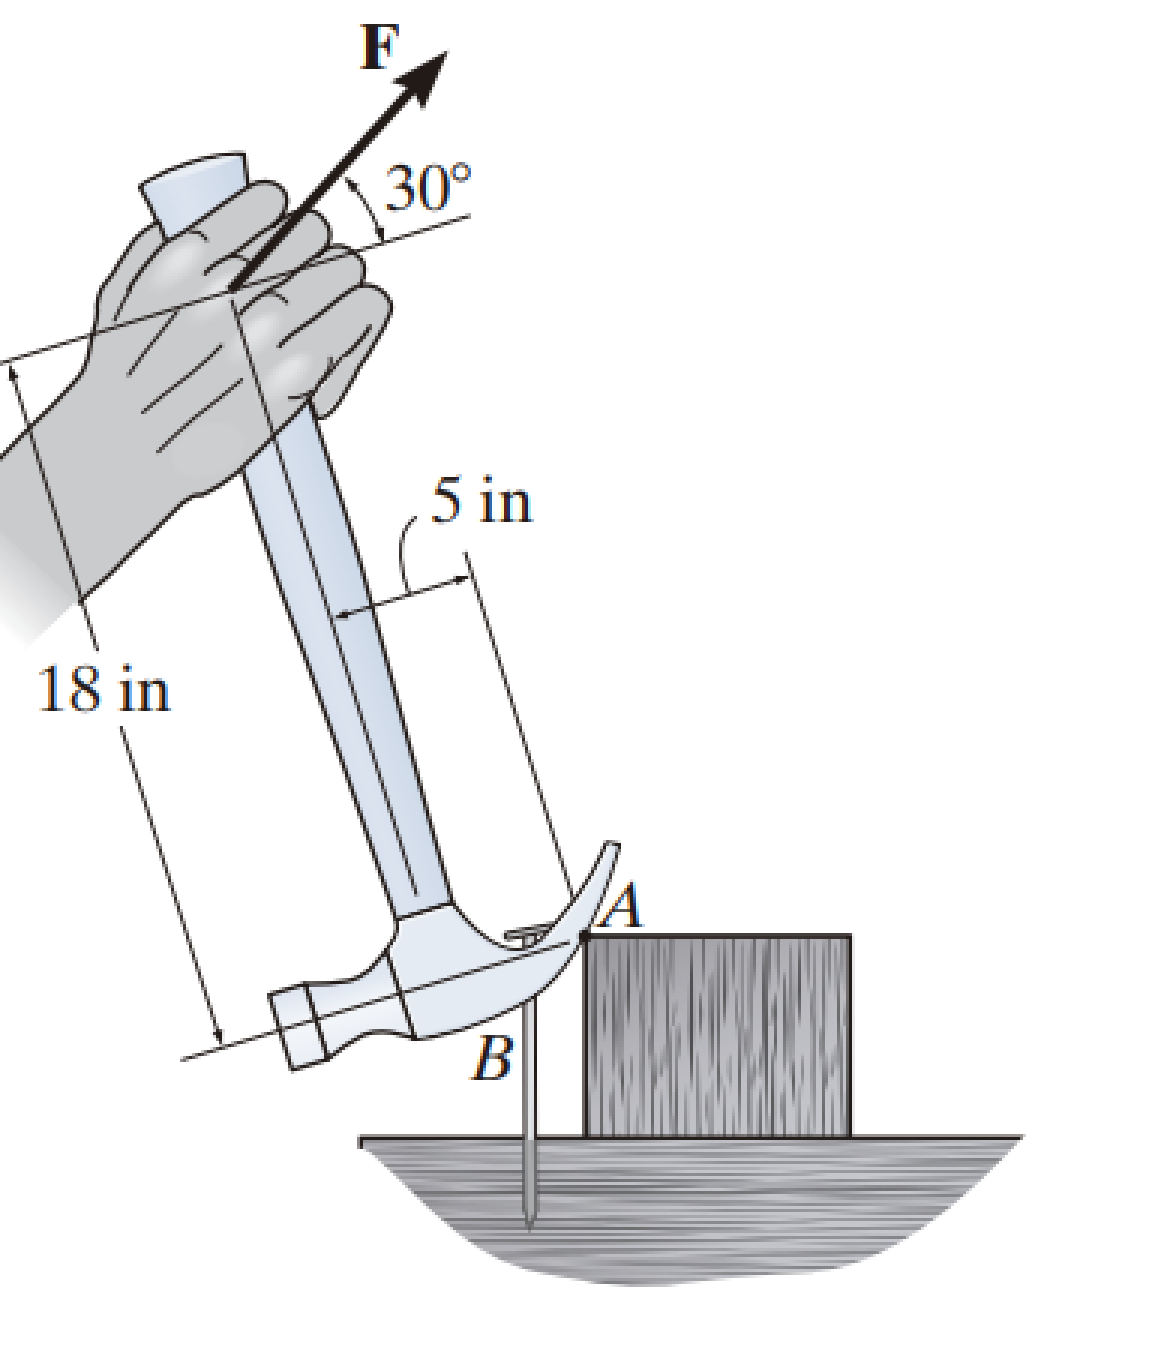
\includegraphics[scale=0.3]{es17.png}
	\caption{Problema 12}
\end{figure}

\textit{ Sol.}

El momento máximo se va a dar cuando el brazo del momento y la fuerza sean perpendiculares entre sí, haciendo un diagrama de un triángulo pitagórico, la base del brazo y el ángulo formado se extrae que:

\begin{align*}
	 & z=\tan{\theta}                                               &  & y=\frac{8}{\cos{\theta}} \\
	 & 10m=z+y=\frac{8}{\cos{\theta}}=10\cos{\theta}-\sin{\theta}=8
\end{align*}

\begin{align*}
	 & (M_5)_{Max}=6\cdot 8=48 KN\cdot m                                                        \\
	 & \overline{BD}=\sqrt{1^2+10^2}=\arctan{\frac{1}{10}}=5.7^{\circ}                          \\
	 & \sin{\alpha}=\frac{1}{\sqrt{101}}\land \cos{\alpha}=\frac{10}{\sqrt{101}}                \\
	 & \frac{10\cos{\theta}-\sin{\theta}}{\sqrt{101}}=\frac{8}{\sqrt{101}}=\frac{8}{\sqrt{101}} \\
	 & \cos{\theta+\alpha}=\frac{8}{\sqrt{101}}=37.24^{\circ}                                   \\
	 & \theta37.24-5.71=31.53
\end{align*}



\begin{problem}
El bastidor en forma de $A$ se eleva hasta la posición erguida, mediante la fuerza vertical de $F=80 lb$. Determine el momento de esta fuerza con respecto al eje $y$ ¿Qué pasa por los puntos $A$ y $B$, cuando el bastidor se encuentra en la posición indicada.
\end{problem}

\begin{figure}[h!]
	\centering
	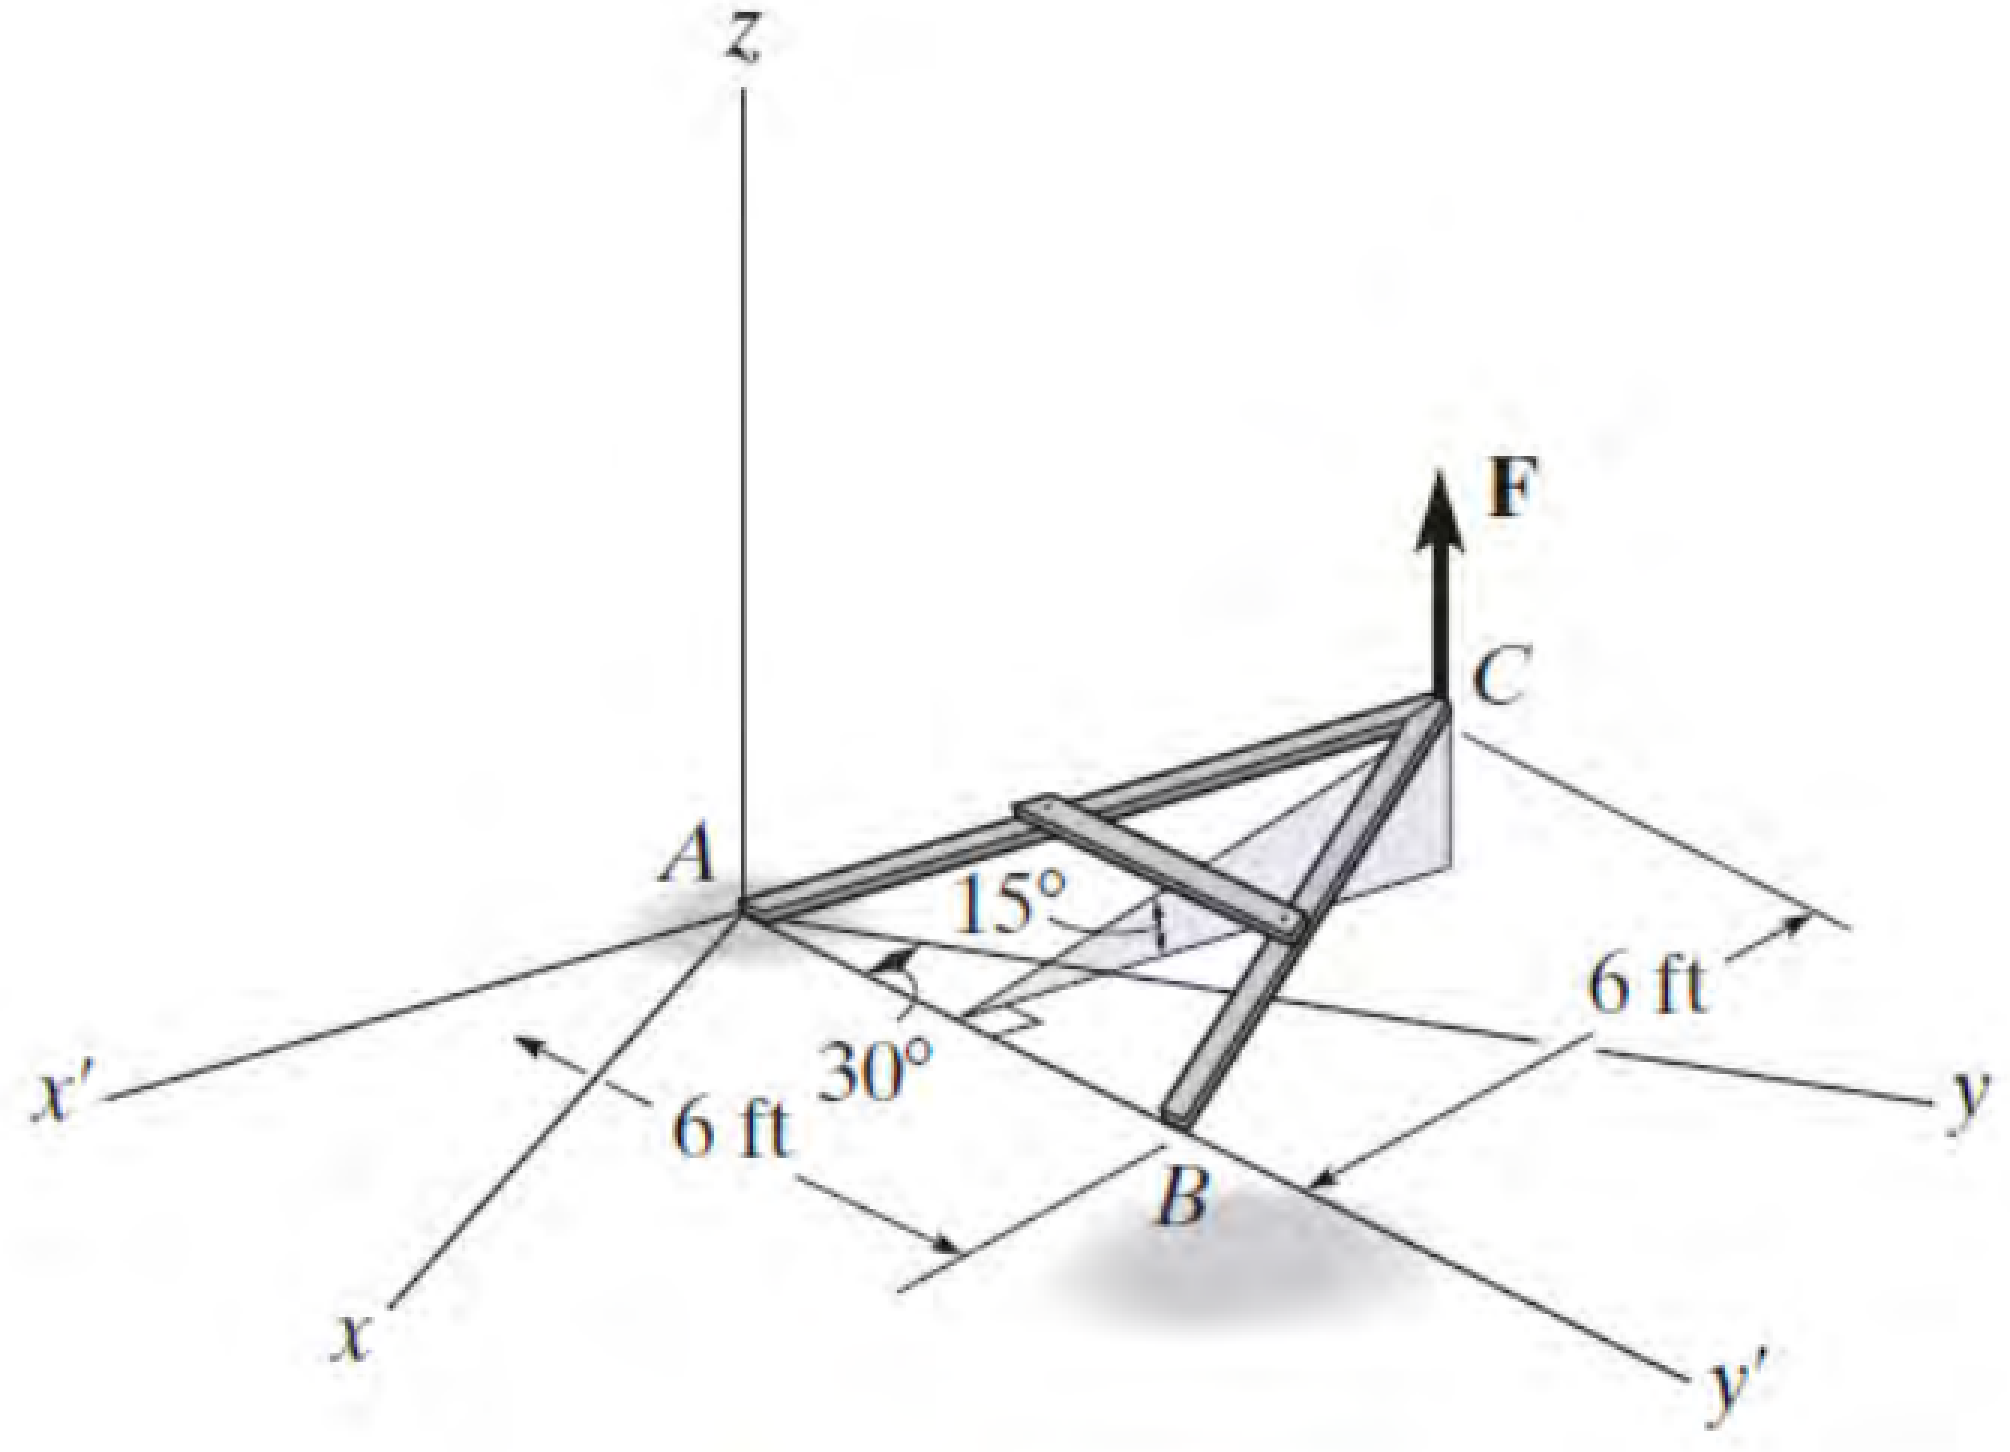
\includegraphics[scale=0.3]{es18.png}
	\caption{Problema 54}
\end{figure}

\textit{ Sol.}

\begin{align*}
	 & M_Y=\vec{M_Y}\cdot(\vec{r_F}\times \vec{F})                                                                                                                                          \\
	 & \vec{r_{AC}}=\vec{r_c}-\vec{r_A}                                                                                                                                                     \\
	 & \vec{AC}=-60\cos{15}i+3j+6\sin{15}k                                                                                                                                                  \\
	 & \vec{F}=F\cdot \vec{U_F}=80lb\cup{K}                                                                                                                                                 \\
	 & \vec{U_Y}=-\sin{30^{\circ}}i+\cos{30^{\circ}}j                                                                                                                                       \\
	 & \begin{bmatrix}
		   -\sin{30^{\circ}} & \cos{30^{\circ}} & 0^{\circ} \\-6\cos{15^{\circ}}&3&6\sin{15^{\circ}}\\0&0&80
	   \end{bmatrix}= \\
	 & -\sin{30^{\circ}}[3(80)-0]-\cos{30^{\circ}}[(-6\cos{15})(80)-0]+0                                                                                                                    \\
	 & M_Y=-120+401.53+0=281.53lbft
\end{align*}

Finalmente el momento en la fuerza vertical es de $281.53 lbft$

